\section{The Dispa-SET model}

\subsection{Overview}

The Dispa-SET model \cite{dispaset} is described in the source \cite{dispaset2} as "an open-source unit commitment and optimal dispatch model focused on the balancing and flexibility problems in European grids".

More precisely, it is focused on simulating large scale power systems, with emphasis on high shares of VRES. As such, it is used as tool for the analysis of the impacts of VRES on the power systems, thank to its ability to take into account several technical constraints of the power system.

A schematic of the Dispa-SET architecture is displayed in Figure \ref{dispaset-architecture}.

\begin{figure}[h]
    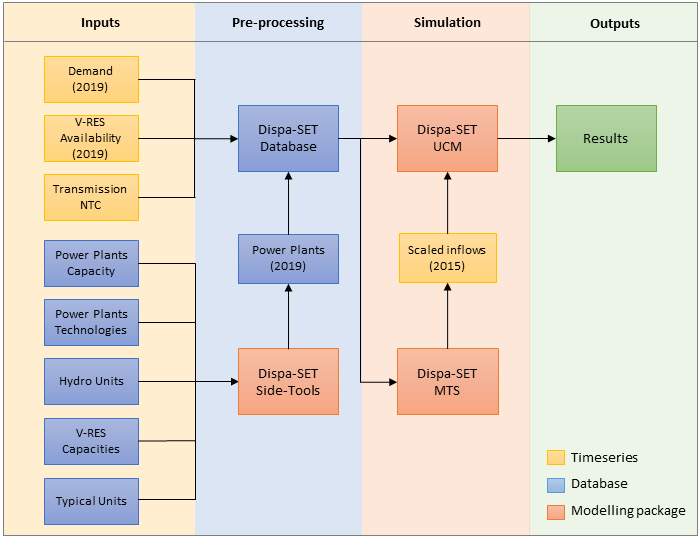
\includegraphics[width=0.9\textwidth]{dispaset-architecture.png}
    \caption{Block diagram of the architecture of the Dispa-SET model}
    \label{dispaset-architecture}
\end{figure}

Its interface is written in the Python programming language, and calls GAMS \cite{GAMS} as the main solver engine.

\subsection{Objective function}

The Dispa-SET model aims at minimizing the overall operating costs of the grid, that is its objective function in this context. These costs typically include transportation, power and heating costs required to split efficiently the demand between the available generation units.

The total system costs is split as follows:
\begin{itemize}
    \item \textit{Fixed cost}: fixed amount, charged if the unit is on.
    \item \textit{Variable costs}: amount that is a function of the power output the units are operating at.
    \item \textit{Start-up} and \textit{Shutdown costs}: amount charged on start and on shutdown of a unit.
    \item \textit{Ramp-up} and \textit{Ramp-down costs}: costs due to the increase or decrease in power output of a unit.
    \item \textit{Shed load costs}: costs due to necessary load sheddings.
    \item \textit{Loss of load costs}: due to generated either exceeding the demand, or not matching it .
    \item \textit{Transmission costs}: due to the use and wear of the transmission network.
    \item \textit{Spillage costs}: due to spillage in storage units.
\end{itemize}

We can formulate, Equation \ref{obj-function-sum} to represent the objective function, where $u$ refers to the index on each units, $i$ is the time index, and $n$ the zone index.

Table \ref{tab:equations-nomenclature} summarizes all the names appearing in the equations.

\begin{table}
    \centering
    \begin{tabular}{|p{0.33\textwidth}|p{0.6\textwidth}|}
        \hline
        Symbol & Meaning \\ \hline
        $Cost[StartUp|ShutDown]_u$ & Cost of the start up or shut down of unit $u$ \\
        $CostRamp[Up|Down]_u$ & Cost of the ramping up or down of unit $u$ \\
        $Cost[Fixed|Variable]_u$ & Fixed or variable cost of operating unit $u$ \\
        $Commited_u$ & 1 if unit $u$ is turned on, else 0 \\
        $Power_u$ & The power unit $u$ operates at \\
        $TimeStep$ & The duration of one simulation time step \\
        $CostLoadShedding_n$ & Cost of the load shedding in zone $n$ \\
        $ShedLoad_n$ & The amount of load being shed in zone $n$ \\
        $LostLoad$ & Lost load, i.e., load that is neither produced, nor accounted as load shedding \\
        $VOLL$ & Value of lost load, i.e., its price per MWh \\
        $CostOfSpillage$ & Cost of spillage in storage units \\
        $Spillage_s$ & Amount of spillage in storage unit $s$ \\ \hline
        $Location_{u,n}$ & Boolean, 1 if unit $u$ is in zone $n$, else 0 \\
        $Flow_{l,n}$ & The electric flow between zones $l$ and $n$ \\
        $Demand_n$ & The demand in zone $n$ \\
        $StorageInput_s$ & The power being inputted into the storage unit $s$ \\ \hline
    \end{tabular}
    \caption{Description of the variables used in Equations \ref{obj-function-sum} and \ref{supply-demand-balance-equation}}
    \label{tab:equations-nomenclature}
\end{table}

\begin{captionnable}[h]
    $Min_{TotalSystemCost}=$
    \begin{equation}
        \begin{split}
            & \sum_{u,i} (CostStartUp_{u,i} + CostShutDown_{u,i}) \:+ \\
            & \sum_{u,i} (CostRampUp_{u,i} + CostRampDown_{u,i}) \:+ \\
            & \sum_{u,i} CostFixed_{u}\cdot Comitted_{u,i} \cdot TimeStep\:+ \\
            & \sum_{u,i} CostVariable_{u,i} \cdot Power_{u,i} \cdot TimeStep\:+ \\
            % & \sum_{u,i} CostVariable_{u,i} \cdot Heat_{u,i} \cdot TimeStep \:+ \\
            & \sum_{n,i} CostLoadShedding_{n,i}\cdot ShedLoad_{n,i} \cdot TimeStep \:+ \\
            % & \sum_{chp,i} CostVariable_{chp,i}\cdot CHPPowerLossFactor_{chp,i}\cdot Heat_{chp,i} \cdot TimeStep \:+  \\
            & \sum_{n} VOLL \cdot LostLoad \cdot TimeStep \\
            % & \sum_{i,n} VOLL_{Power}·(LostLoad{MaxPower,i,n} +LostLoad{MinPower,i,n}) \cdot TimeStep \:+  \\
            % & \sum_{i,n} 0.8 \cdot VOLL_{reserve}·(LostLoad{2U,i,n} + LostLoad{2D,i,n} + LostLoad{3D,i,n}) \cdot TimeStep \:+ \\
            % & \sum_{u,i} 0.7 \cdot VOLL_{Ramp}·(LostLoad{RampUP,u,i} +LostLoad{RampDown,u,i}) \cdot TimeStep \:+\\
            & \sum_{s,i}CostOfSpillage \cdot Spillage_{s,i}
        \end{split}
        \label{obj-function-sum}
    \end{equation}
    \equationcaption{Objective function of the Dispa-SET model}
\end{captionnable}

\subsection{Supply and demand balance}

At all time and in each zone, the fundamental constraint that has to be met is the supply-demand balance in terms of energy production (supply) and consumption (demand), in the day-ahead market.

The supply sources are:
\begin{itemize}
    \item The power outputs from each units 
    \item The power outputs from storage units discharging
    \item The (eventual) net income from importation from neighbouring zones
    \item The (eventual) shed load
\end{itemize}

Whereas the demand originates from:
\begin{itemize}
    \item The load in that zone
    \item The (eventual) net exportations to neighbouring zones
    \item The power consumed by charging storage units
    \item The power consumed by P2H (power to heat) units
\end{itemize}

Equation \ref{supply-demand-balance-equation} expresses this target energy production and consumption balance.

\begin{captionnable}[h]
    \begin{equation}
        \begin{split}
            &\sum_{u} (Power_{u,i} \cdot Location_{u,n}) + \sum_{l} Flow_{l,n,i} \\
            & = Demand_{n,i} + \sum_{s} (StorageInput_{s,i} \cdot Location_{s,n}) + \\
            % & \sum_{p2h}(PowerConsumption_{p2h,i} \cdot Location_{p2h,i}) - ShedLoad_{n,i} - LostLoad 		
            & - ShedLoad_{n,i} - LostLoad 		
        \end{split}
        \label{supply-demand-balance-equation}
    \end{equation}
    \equationcaption{Supply-demand balance in Dispa-SET}
\end{captionnable}

\subsection{Rolling horizon}

The ideal solution would be to solve the entire system, for every time step in the complete duration of the simulation in one go. But this would create a system too large to be efficiently solved.

To address this, the UCM simulation is split into smaller, tractable parts. The simulation is built for smaller time frames, called optimization periods, over which the simulations can be made easily.

The start of optimization period $j$ overlaps the optimization period $j-1$, to that the simulation $j$ is the correct prolongation of the same setting fixed by the simulations up to $j-1$. The period that overlaps is called the look-ahead, in which the values of the parameters for period $j-1$ is determined during simulation $j-1$, and are used as fixed context for simulation $j$. A depiction of rolling horizon is given in Figure \ref{fig:rolling-horizon}.

\begin{figure}[h]
    \centering
    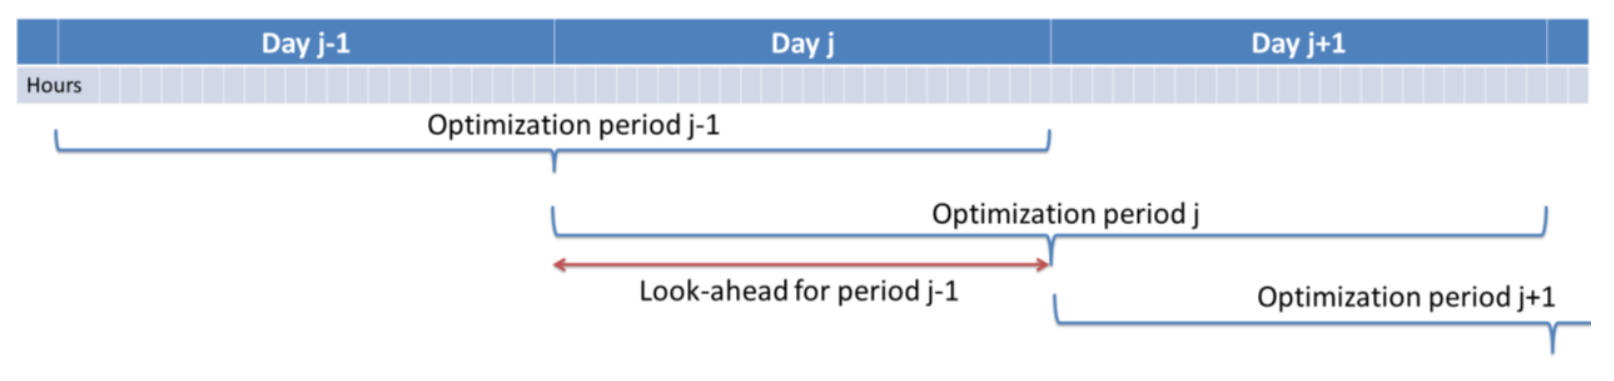
\includegraphics[width=0.9\textwidth]{resources/images/rolling_horizon.png}
    \caption{Depiction of the rolling horizon mechanism}
    \label{fig:rolling-horizon}
\end{figure}

\subsection{Mid-term scheduling}

Without further constraints, the optimization will most often leave all storage facilities empty at the end of the simulation horizon (typically a few days). This is a consequence of the variable operational cost of discharging these storage units being smaller than the cost of running another unit, thus charging extra fixed and variable costs.

To address this issue, the Dispa-SET model has to be run in Mid-Term Scheduling (MTS) mode. In this mode, the initial and final levels of the storage units (in particular, pumped hydro storage units) are given as exogenous input to the model. These levels are enforced with additional constraints.

However, this options has additional requirements. The formulation has to be set to LP, the rolling horizon is turned off and the time resolution is risen to one day.

In this work, the MTS mode is enabled, and the exogenous inputs, for both initial and final levels, are set to half of the storage capacity.

\subsection{Problem formulations}

Dispa-SET features several, different formulations, with a significant impact on the realism and accuracy of the output. These formulation differ in the way the simulation is created and the constraints defined.

\subsubsection{Linear programming}

In the LP formulation, every variable is considered to be continuous, and can take values continuously down to zero. In particular, this applies to the $Commited$ variable, hence enabling any power output from 0 to the unit's maximum power.
% In particular, this constraint applies to the power output of each unit, that is, the ratio of the actual power the unit is operating over its maximum capacity. Therefore, as a unit cannot produce more than its maximum capacity, this value must lie in the $[0, 1]$ interval at every hour of the simulation.

However, the LP formulation lacks the capacity to enforce minimum operating levels for units effectively, leading to potentially unrealistic scenarios, for example a nuclear unit operating at 10\% of its maximal power, what is not achievable.

\subsubsection{Binary formulation}

To mitigate this issue, the $Commited$ variable is made boolean. That way, the minimum operating value can be enforced when the corresponding commited boolean is set to one.

This strategy, however achieving the better accuracy targetted, is unfortunately often intractable in realistic settings, due the large number of binary variables (one for each unit) yielding an exploding number ($2^N$) of options to be examinated.

\subsubsection{Mixed integer linear programming \label{subsubsection:milp}}

The MILP formulation is created to leverage the computational cost of the simulation while keeping a good level of accuracy. The main idea is to group the units that share similar properties together, and only keep track of the number of units in each group that are currently commited.

This permits the number of options to explore reasonnable, without hurting the precision of the output.

In this work, the MILP formulation is chosen due to its better efficiency-to-computational-cost trade-off.

\subsection{Reference simulation \label{section:reference-simulation}}

This work takes the simulation over the year 2019 as a reference. Accordingly, the several input timeseries, including the demand, the availability factors, and the flows between each zones are used.

Dispa-SET also detects congestion issues. These appear when a link transmits too much power for its capacity. For electric wires, congestion causes a wire to retain heat, what may threaten the wire integrity. While seemingly harmless, this phenomenon is likely to be on the rise, for example when an area produces a lot of renewable energy, and has to transmit it to some neighbour in deficit.

The annual dispatch plot generated by Dispa-SET for the reference simulation in Belgium is displayed in Figure \ref{fig:dispatch-be}.

\begin{figure}[h]
    \centering
    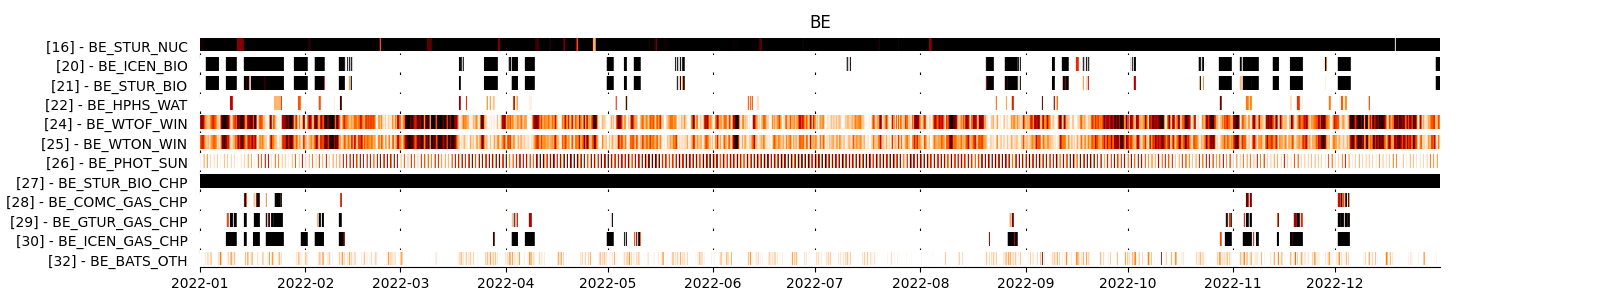
\includegraphics[width=0.8\textwidth]{resources/images/commited-BE-year.png}
    \caption{Dispa-SET reference simulation. Commited units over one year in Belgium}
    \label{fig:dispatch-be}
\end{figure}

The observations drawn from Figure \ref{fig:dispatch-be} are as follows:
\begin{itemize}
    \item The units "BE\_STUR\_NUC" and "BE\_STUR\_BIO\_CHP" are almost always on. These correspond to turbines powered by nuclear energy and bio fuels respectively. The latter is a combined heat and power unit.
    \item Wind turbines, both on-shore and off-shore, have roughly the same availabilities.
    \item The higher availability in PV energy during summer is apparent, along with the day-night cycle.
    \item Other units like "BE\_ICEN\_BIO", "BE\_STUR\_BIO", "BE\_GTUR\_GAS\_CHP" and "BE\_ICEN\_GAS\_CHP" seem to be turned on while wind units generate less power, especially during winter.
\end{itemize}

Figure \ref{fig:dispatch-de-week} presents a dispatch plot over a week in Germany.

\begin{figure}[h]
    \centering
    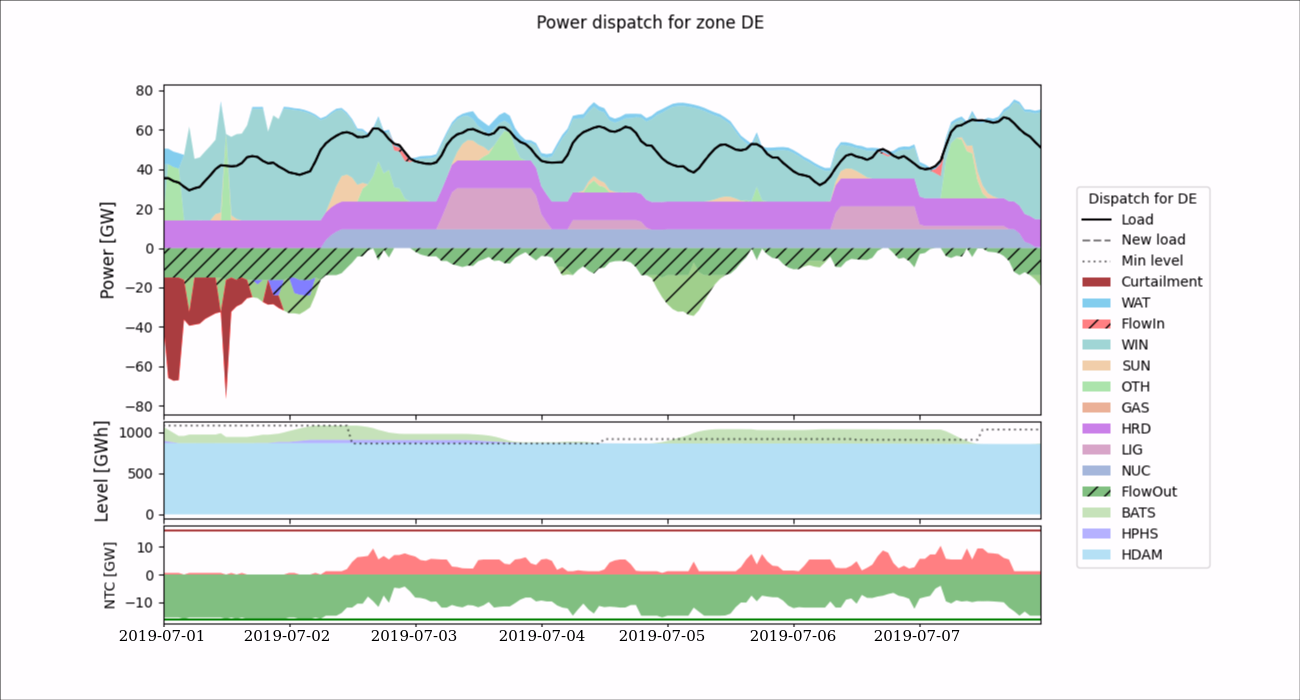
\includegraphics[width=0.8\textwidth]{resources/images/dispatch-DE-week.png}
    \caption{Dispa-SET reference simulation. Dispatch plot over a week in Germany}
    \label{fig:dispatch-de-week}
\end{figure}

In Figure \ref{fig:dispatch-de-week} we first observe some curtailment in the first day, indicated by the red area. The green striped region indicates that the zone was exporting excess production during the week. This is aligned with the depicted NTC, presenting a greater flow outwards than inwards. Moreover, the reservoirs of storage units were predominantly full. As the demand was entirely met by the production, no load shedding appeared. In the latter case, the load curve would be higher than the production and importations sum.